\clearpage
\section*{S24. Fixed-current-dimension definitions and reproducible selectors}
The common forward state is full-wave; only tangent currents are reduced. The real material normal equation retains the physical prior gradient $\ell$, regularizer/damping $\Lambda$, and exact polarizability derivative. The actual complex current rank is shared across illuminations, not a real material rank. All tested spaces meet the prescribed $k$ or are recorded as infeasible. Reference and reduced true-normal residual limits are $10^{-10}$ and $10^{-8}$; the largest recorded admitted values are $9.5472\times10^{-12}$ and $9.3829\times10^{-10}$. The current rank and relative compressed singular-value limits are $10^{-10}$, with no hidden ridge.

The finite and first-order selectors use a common independently built 64-column current reference and common candidates. They retain full Schur coupling and rescore after each addition. The finite rule includes the quadratic cost of the proposed material-step change; the first-order rule omits it. Fixed lookahead and swap limits are inherited from the development lock. The limited-probe variant has only its declared complete-model action permission. Its information acquisition and rejected work are charged even if its result coincides with the no-probe version.

The generic control is an adaptation of primal--dual current POD/Galerkin: anchor material steps for the measured residual and four fixed normalized scenarios produce primal and dual current responses. The two blocks have equal trace weight before a total-$k$ shared-space POD; fixed completion supplies missing rank. It is not a reproduction of an entire interpolatory inverse-ROM optimizer. The receiver/internal control uses the projected complementary receiver construction described in Chen's book, with an approximate internal right-singular basis. It is not native nonlinear TSOM, FFT-TSOM, or their exact-intersection formulation.

The offline current search operates on the union of the fixed dictionary and evaluated legitimate baseline spaces, including deployed selector spaces, before bounded multistart/swap proposals. It is not globally certified. Material-only low-rank controls and unrestricted full-step current witnesses have separate records and do not enter that oracle domain or equal-current-budget statistics.

\section*{S25. Conditional noiseless coverage and complete control readings}
The original design has 16 objects, three states, and seven noise realizations per state: 336 instances and 2016 state--budget cells per method. Unstarted 1\%/3\% noise tests were explicitly deferred, retaining 288 instances/1728 cells. The conditional noiseless target is 48 instances/288 cells. Admission accepts 43 instances/258 cells and 5418 current-method records; ten random seeds remain distinct methods, not distinct objects. One reference failure removes three states and two native process failures remove one state each. No gap is replaced with zero, another object, or a copied state. The interrupted old state is excluded; its separately authorized optimized result is admitted once.

Thirteen objects have all states, two have two states, and one has no reference. All primary results use the 15 observed objects. A separate complete-three-state sensitivity gives finite/receiver ratio 1.0947, finite/primal--dual ratio 0.2904 and regret 1.1396, unchanged at the reported precision. Its offline-search ratio is 0.3214; this sensitivity does not replace the primary 0.4242 estimate.

The primary object ratio sums matched absolute gaps within each object before division; the overall estimate is the median object ratio. Intervals use 10,000 clusters with seed 20260930. Reference floors are fixed from reference normal residual and FP64 roundoff. Opportunity capture is evaluated only when receiver gap minus same-domain search gap exceeds the common floor: 256 units qualify. Regret is the object ratio of summed finite-minus-search to summed receiver-minus-search gaps; capture is one minus regret. Raw negative capture is retained. No ordering violation below the floor is observed. Full-quadratic gap uses the stable $H$-energy formula with the measured reference-gradient linear remainder, rather than subtracting two nearly equal objective values blindly.

\begin{table}[htbp]\centering\caption{All nonrandom current-selection controls: object-median full-quadratic gap ratio versus the locked receiver rule, over the conditional observed noiseless subset. This table is not a native algorithm comparison.}\begin{tabular}{lr}\toprule
Selection rule & Ratio\\\midrule
Receiver singular vectors & 1.000000\\
Projected receiver/internal proxy & 15.014409\\
Fourier directions & 25.265358\\
Current-energy POD & 18.300646\\
Raw two-sided transfer magnitude & 7.148301\\
Joint spectrum with actual current lifting & 224.022912\\
First-order signed gain & 7.393912\\
Finite gain, no full probes & 1.094721\\
Finite gain, limited full probes & 1.094721\\
Adapted primal--dual POD/Galerkin & 3.516725\\
Offline best-found current search & .424190\\\bottomrule
\end{tabular}\end{table}

The aggregate no-probe ratios by family are 1.3481 (Gaussian lobes), 1.0796 (contact), 1.5843 (shell/layered), and 0.2793 (asymmetric). The ratios by material representation are 1.5090 (seven Gaussian objects) and 0.8724 (eight voxel objects). Initial, middle and final-state ratios are 1.2761, 0.2793 and 0.3597. All are descriptive prespecified slices; neither incomplete coverage nor failed aggregate criteria is overridden by favorable slices.

\begin{figure}[htbp]\centering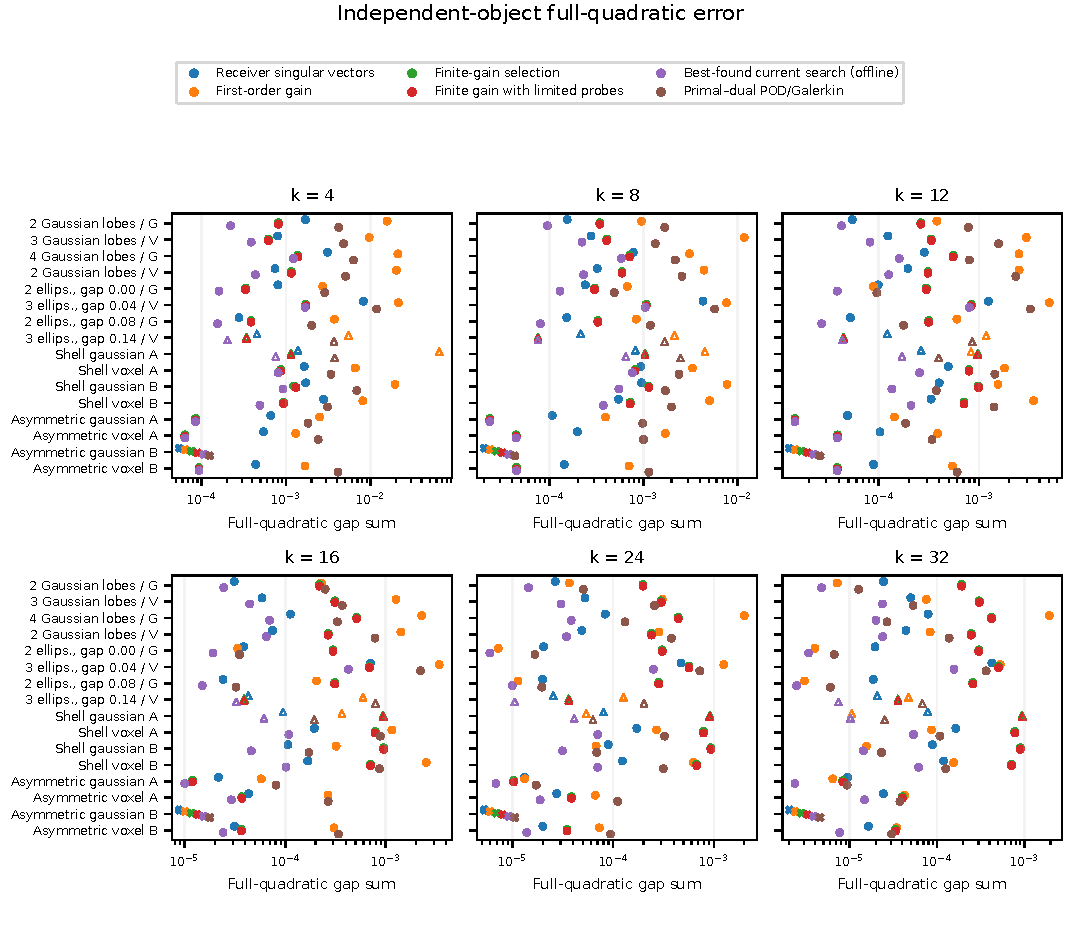
\includegraphics[width=.98\linewidth]{figures/current_design/02_object_fullgap.pdf}
\caption{Observed absolute full-quadratic gaps at all six budgets and all 16 planned objects. Filled/open markers distinguish complete/partial state coverage; missing objects have annotations rather than numerical zero. Object names describe geometry and material representation. Different objects are not points along one physical trajectory.}
\end{figure}
\begin{figure}[htbp]\centering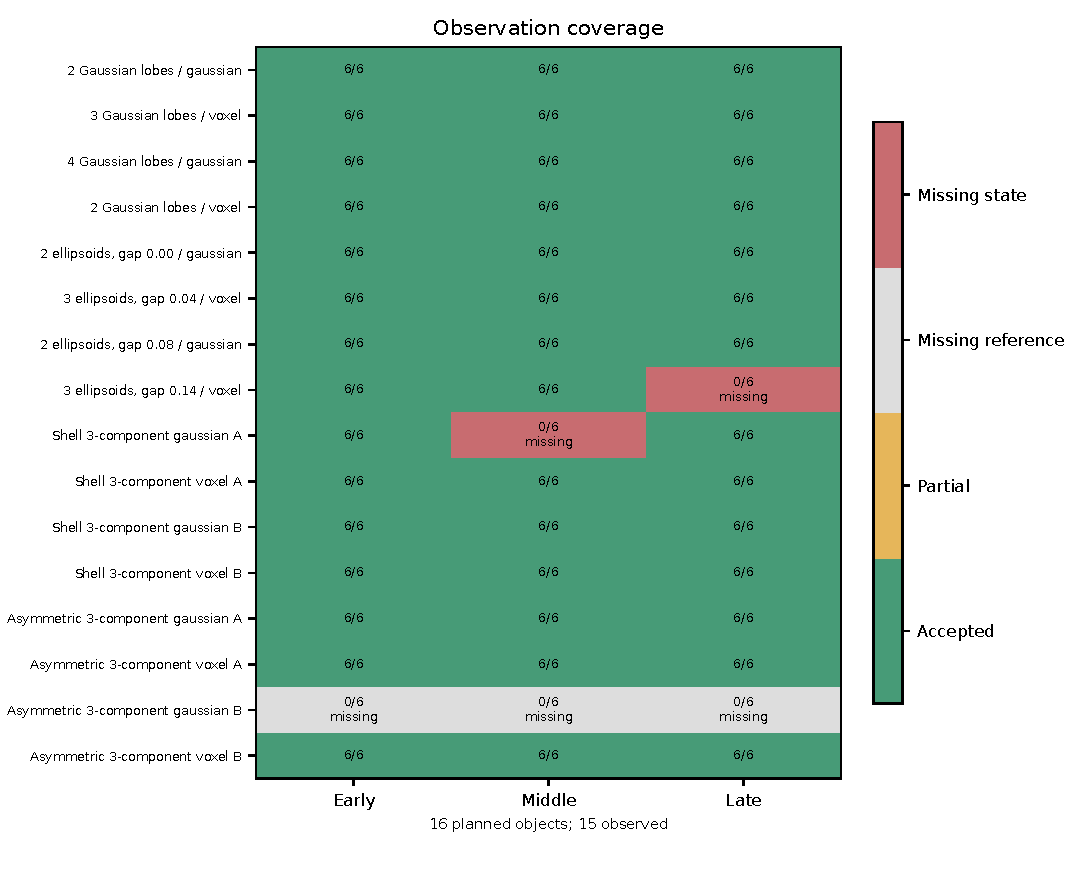
\includegraphics[width=.92\linewidth]{figures/current_design/04_zero_coverage.pdf}
\caption{Every planned noiseless state remains visible, including the failed reference and native process gaps. This conditional 43/48-state coverage does not close the original noise-inclusive gate.}
\end{figure}

\section*{S26. Information, cost and provenance boundaries}
The complete shared attempt ledger contains 166 uniquely paired starts/ends and 92629.937324\,s occupation (25.730538\,h), including diagnostics, full references, offline evaluation, failed attempts and interrupted work. Eight optimized continuation jobs consume 9086.047\,s. Five use CUDA candidate batches with CPU work retained; three small Gaussian cases use the exact CPU scoring path. Occupation includes host algebra, transfers, saving and waiting within a numerical job; it is not GPU kernel-active time.

\begin{figure}[htbp]\centering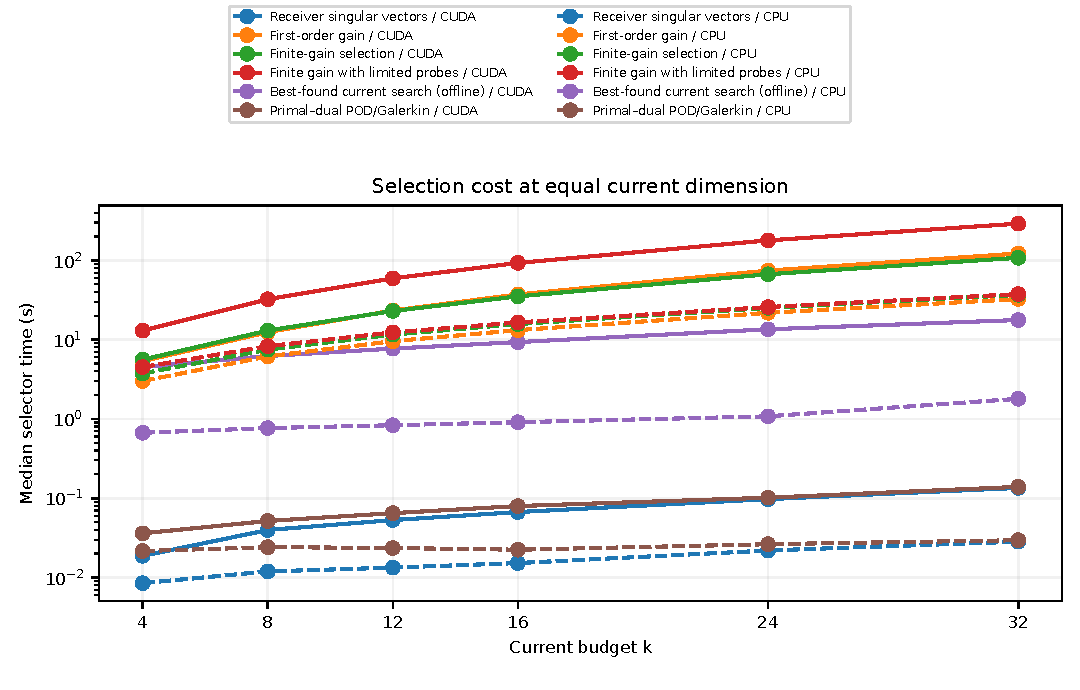
\includegraphics[width=.98\linewidth]{figures/current_design/03_selector_wall.pdf}
\caption{Version-separated shared-workspace marginal selector fees. The five CUDA-batched and three exact-CPU cases differ in object and material dimension, so these curves do not establish a cross-backend speedup. The older backend is not uniformly recorded and remains in the cost tables. Common-bank construction, reference, offline and interrupted work are separately charged; natural cold-deployment time is unmeasured.}
\end{figure}

The interrupted state retains 218 partial files and its uncertain-exit occupation upper bound of 1376.604324\,s. Failed native/reference attempts remain paid. All 46 core-validation source declarations match; seven of 15 earlier development declarations have an open historical source-version gap. One failed late-state setup component is missing, but its attempt fee is present. Cold/no-history/minimal-natural totals are unmeasured. Overlapping counter views are not summed twice.

The terminal archive binds old/optimized outputs, locks, configuration, material bases, reference authorities and attempts. Its SHA256 is
\par\noindent{\footnotesize\ttfamily ce31e9104fd25589207ee50e84dce9973525b39db0c991d20695ae82bab0e130}\par
Original seals and the external pre-first-selection authority for two unused references are retained with native/local mappings. Old records remain unchanged. Original SOM/TSOM/FFT-TSOM/S-DBIM publication-source gaps stay open.

Overall risk, cross-family/budget benefit, object wins and oracle capture fail their aggregate criteria. Only the adapted primal--dual comparison meets its conditional numerical threshold. Large-grid causal interventions, noise checks and selector reconstruction have no new results. The paper retains its mechanism and design-condition positioning.
